Di seguito vengono spiegati l'utilizzo degli strumenti di modifica delle presentazioni.

\subsection{Layout principale}
Una volta avviato l'editor delle presentazioni la pagina che appare si presenta semplice ed intuitiva. A sinistra si trova un menù verticale con tutti i pulsanti che permettono di modificare la slide\ped{G} corrente. Al centro dello schermo invece si trova lo spazio di gestione dei contenuti della slide\ped{G}, dove è possibile interagire con i contenuti. In alto a destra si trova il pulsante verde per l'avvio dell'aiuto a schermo.

\begin{figure}[H] 
	\centering 
	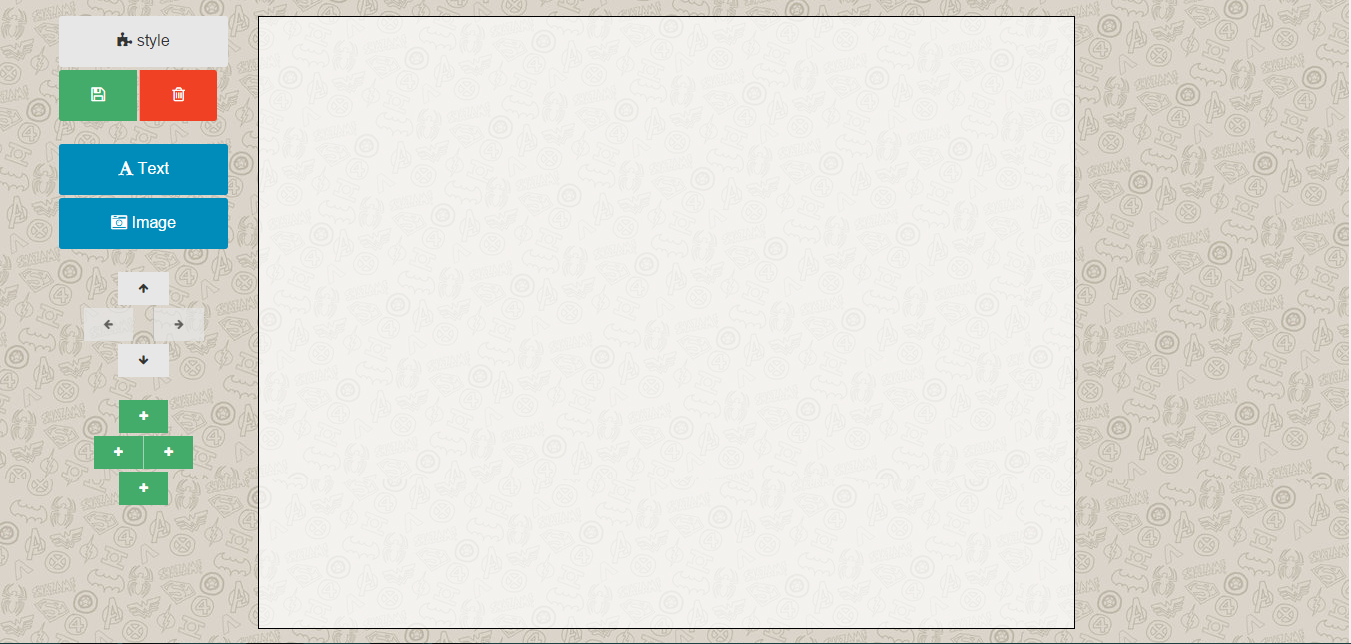
\includegraphics[scale=0.40] {img/layout_editor.png}
	\caption{Layout principale} 
\end{figure}

\subsection{Visual Help}
Il pulsante posto in alto a destra, di colore verde, \textbf{Visual Help} permette l'avvio di un breve tour guidato, che mostra mediante l'utilizzo di pop-up\ped{G} le varie funzionalità associate ai pulsanti presenti nella schermata di modifica delle presentazioni. Una volta premuto il bottone, apparirà sullo schermo un piccolo pop-up\ped{G} di colore nero con una breve spiegazione sulle funzionalità del pulsante indicato dal pop-up stesso (come il pulsante viene indicato dal pop-up\ped{G} è segnalato nell'immagine sottostante):

\begin{figure}[H] 
	\centering 
	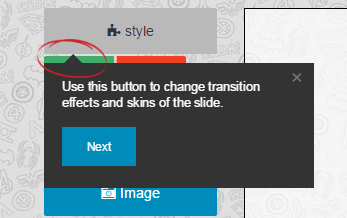
\includegraphics[scale=0.80] {img/tour.png}
	\caption{Visual Help - Pop-up di aiuto del pulsante Style} 
\end{figure}


\subsection{Menù laterale di sinistra}
Di seguito verrà analizzato, dall'alto verso il basso, ciascun pulsante presente nel menù laterale di sinistra.

\begin{itemize}
 \item \textbf{Style}\\
    Il pulsante \textbf{Style} permette di scegliere gli effetti di transizione e il tema da applicare alla slide\ped{G}. Una volta scelte le modifiche si deve confermare con il tasto \textbf{OK}.	
    \begin{figure}[H] 
    	\centering 
    	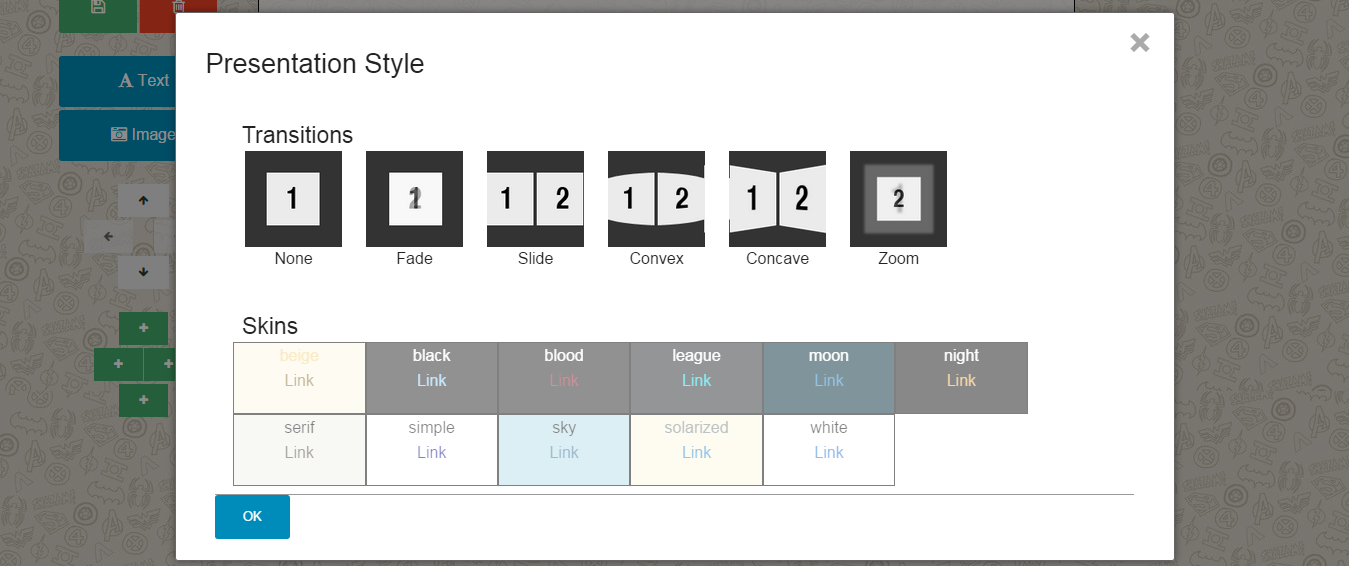
\includegraphics[scale=0.40] {img/editor_style.png}
    	\caption{Menù laterale - Style} 
    \end{figure}
	
 \item \textbf{Salva}\\
	Il pulsante di colore verde è il pulsante che permette di salvare le modifiche apportate alla slide\ped{G}. 	
	\begin{figure}[H] 
		\centering 
		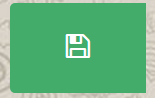
\includegraphics[scale=0.40] {img/editor_save.png}
		\caption{Menù laterale - Salva} 
	\end{figure}
	
	 \item \textbf{Elimina}\\
	 Il pulsante di colore rosso è il pulsante che permette di eliminare tutto il contenuto della slide\ped{G} corrente.  	
	 \begin{figure}[H] 
	 	\centering 
	 	
\includegraphics[scale=0.40] {img/editor_del.png}
	 	\caption{Menù laterale - Elimina} 
	 \end{figure}
	
 \item \textbf{Text}\\
    Il pulsante \textbf{Text} permette di inserire del testo all'interno della slide\ped{G}. Una volta inserito il testo nell'apposita casella si deve confermare con il tasto \textbf{OK}.
    \begin{figure}[H] 
	\centering 
	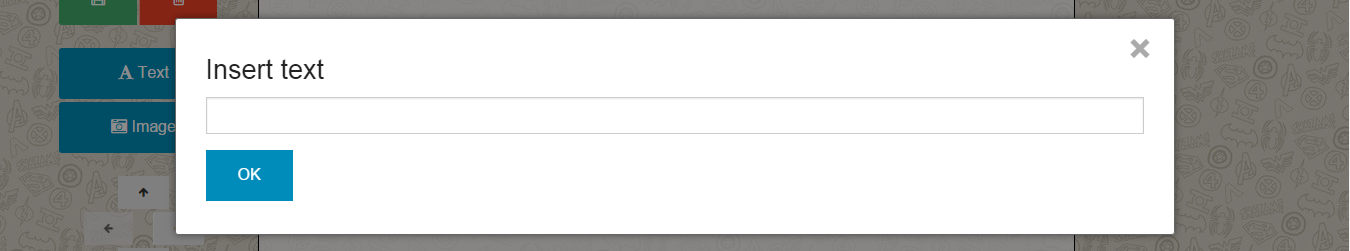
\includegraphics[scale=0.40] {img/editor_text.png}
	\caption{Menù laterale - Text} 
    \end{figure}
    
    
 \item \textbf{Image}\\
    Il pulsante \textbf{Image} permette di aggiungere un'immagine alla slide\ped{G} corrente tra quelle già caricate o di caricarne un'altra presente sul file system\ped{G} dell'utente. Una volta scelta l'immagine, questa verrà inserita automaticamente nella slide\ped{G}.
   \begin{figure}[H] 
	\centering 
	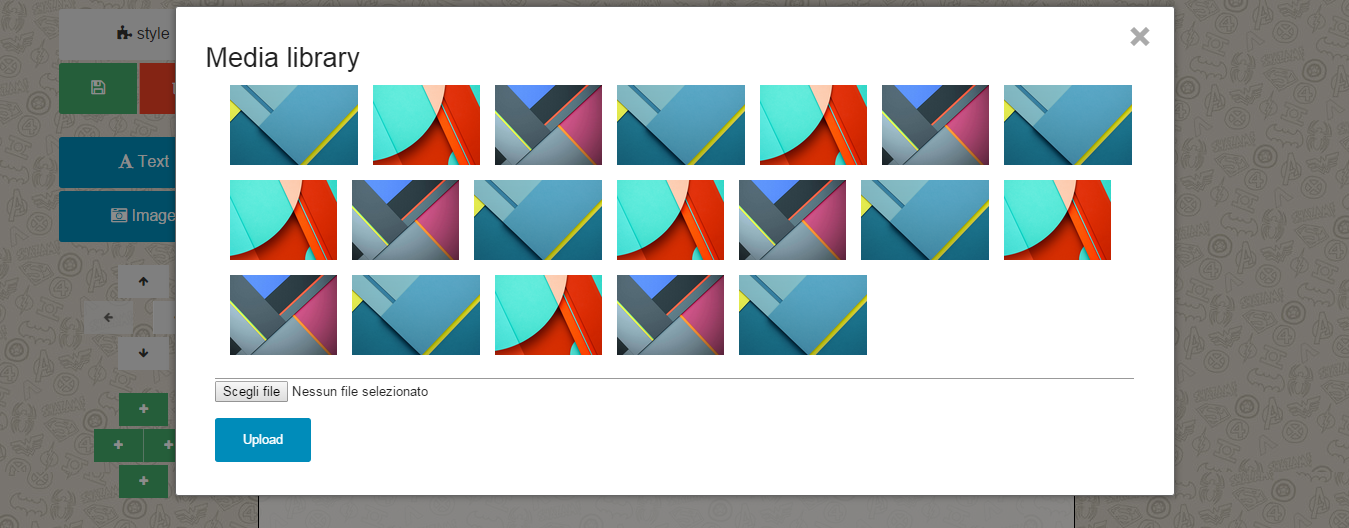
\includegraphics[scale=0.40] {img/editor_img.png}
	\caption{Menù laterale - Image} 
    \end{figure}

  \item \textbf{Table}\\
  Questa funzionalità non è stata ancora implementata.
  
  \item \textbf{Chart}\\
  Questa funzionalità non è stata ancora implementata.
  
  \item \textbf{RealTime}\\
  Questa funzionalità non è stata ancora implementata.


  \item \textbf{Navigazione delle slide}\\
  I pulsanti freccia permettono di navigare tra le slide\ped{G} già create della presentazione. Ad ogni tasto corrisponde una direzione di spostamento.
  \begin{figure}[h] 
  	\centering 
  	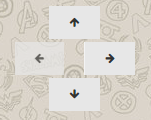
\includegraphics[scale=0.80] {img/editor_move.png}
  	\caption{Menù laterale - Aggiunta di una slide} 
  \end{figure}
 
 
 
\item \textbf{Aggiunta di una slide}\\
 Il pulsante con il simbolo \textbf{+} permette di aggiungere una nuova slide\ped{G} nella direzione corrispondente al pulsante premuto.
 \begin{figure}[h] 
 	\centering 
 	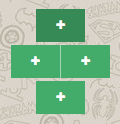
\includegraphics[scale=0.80] {img/editor_add.png}
 	\caption{Menù laterale - Aggiunta di una slide} 
 \end{figure}

\end{itemize}


\newpage

\subsection{Modifica di un componente}
Per modificare un componente è sufficiente selezionarlo nella slide\ped{G} e modificarne gli attributi dal menù che comparirà sulla destra.

\subsubsection{Text}
La grandezza, la posizione e la rotazione della casella di testo possono essere modificate con il mouse tramite gli appositi punti di ancoraggio che compaiono una volta selezionato il testo. Il trascinamento in un angolo provoca una variazione della dimensione proporzionale tra larghezza ed altezza.

\begin{figure}[H] 
	\centering 
	
\includegraphics[scale=0.80] {img/text_anchor.png}
	\caption{Modifica di un componente - Modifica testo con mouse} 
\end{figure}

\noindent In alternativa si possono modificare le proprietà del testo dal menù laterale di destra, nel dettaglio:
		
		\begin{itemize}
			\item \textbf{ScaleX}: modifica la larghezza della casella di testo;
			\item \textbf{ScaleY}: modifica l'altezza della casella di testo;
			\item \textbf{Freccia verso l'alto}: sposta la casella di testo di un livello verso l'alto;
			\item \textbf{Freccia verso il basso}: sposta la casella di testo di un livello verso il basso;
			\item \textbf{Delete}: elimina la casella di testo;
			\item \textbf{Text}: modifica il testo contenuto nella casella di testo;
			\item \textbf{Tasto B}: modifica lo stile del testo in BOLD;
			\item \textbf{Tasto I}: modifica lo stile del testo in ITALIC;
			\item \textbf{Tasto U}: modifica lo stile del testo in UNDERLINE;
			\item \textbf{Size}: modifica la grandezza del testo;
			\item \textbf{Select Font}: modifica il font del testo;
			\item \textbf{Color}: modifica il colore del testo.
		\end{itemize}
		 \begin{figure}[h] 
		    \centering 
		    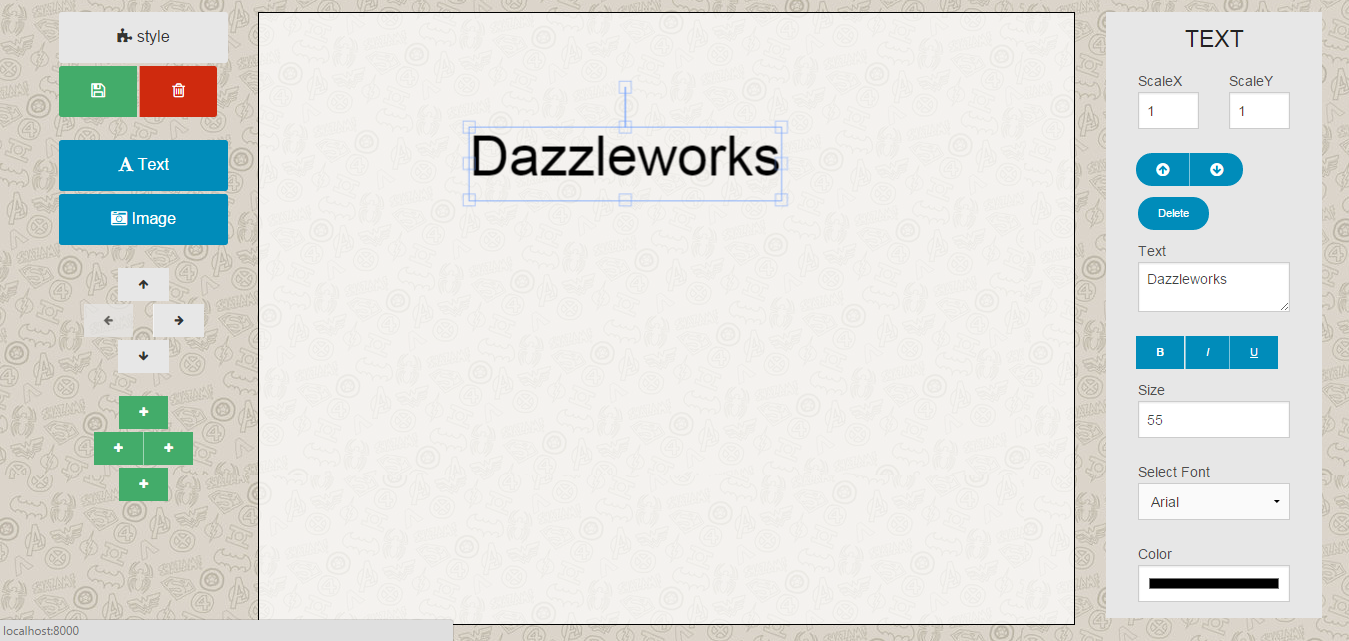
\includegraphics[scale=0.40] {img/text_edit.png}
		    \caption{Slide Editor - Modifica testo da menù} 
		\end{figure}
		
		
\newpage 

\subsubsection{Image}
La grandezza, la posizione e la rotazione dell'immagine possono essere modificate con il mouse tramite gli appositi punti di ancoraggio che compaiono una volta selezionata l'immagine. Il trascinamento in un angolo provoca una variazione della dimensione proporzionale tra larghezza ed altezza.

\begin{figure}[H] 
	\centering 
	
\includegraphics[scale=0.80] {img/img_anchor.png}
	\caption{Modifica di un componente - Modifica immagine con mouse} 
\end{figure}

\noindent In alternativa si possono modificare le proprietà dell'immagine dal menù laterale di destra, nel dettaglio:

		\begin{itemize}
			\item \textbf{ScaleX}: modifica la larghezza dell'immagine;
			\item \textbf{ScaleY}: modifica l'altezza dell'immagine;
			\item \textbf{Freccia verso l'alto}: sposta l'immagine di un livello verso l'alto;
			\item \textbf{Freccia verso il basso}: sposta l'immagine di un livello verso il basso;
			\item \textbf{Delete}: elimina l'immagine;
		\end{itemize}
		
\begin{figure}[H] 
	\centering 
	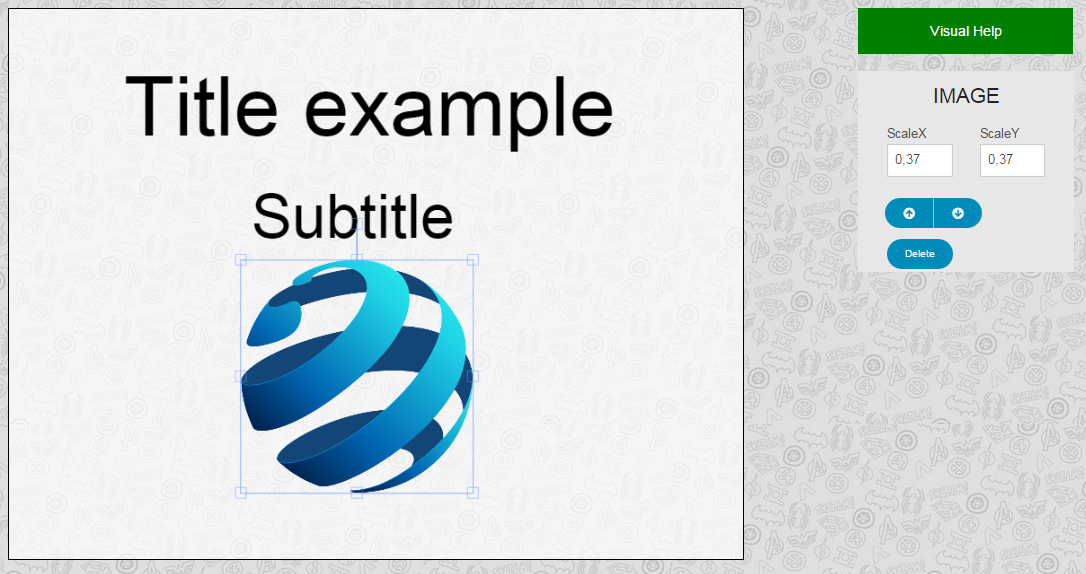
\includegraphics[scale=0.40] {img/img_edit.png}
	\caption{Slide Editor - Modifica immagine da menù} 
\end{figure}	


